
\documentclass[12pt,a4paper]{article}
\usepackage[T2A]{fontenc}
\usepackage[utf8]{inputenc}
\usepackage[english]{babel}
\usepackage[left=2cm,right=2cm,top=2cm,bottom=2cm]{geometry}
\usepackage{cyrtimes}
\usepackage{graphicx}
\usepackage{listings}
\usepackage{indentfirst}
\usepackage{tabularx}
\usepackage{hyperref}
\usepackage{setspace}
\begin{document}
\lstset{
numbers=left,
tabsize=4,
breaklines=true,
title=\lstname,
}
\title{Status report for IMT4002}
\author{(Nataliia Uvarova, Oleksandr Yakushev, 13HMACSA)}
\date{2014}
\maketitle
\onehalfspacing

%----------------------------
\section{Overview}

After considering two service architectures, SOAP and REST, we decided
to go with the latter. Our RESTful service is implemented in Python by
using Flask microframework\footnote{\url{http://flask.pocoo.org/}}.
It greatly simplifies handling HTTP requests and lets focus on the
client side more.

Client-side is written mostly in Javascript together with AngularJS
framework\footnote{\url{http://www.angularjs.org/}}. AngularJS has
many advantages over using plain JS, as it strongly promotes MVC
pattern, supports declarative programming for the UI and allows to
avoid many of the Javascript ugly parts.

Requirement to be able to work while offline is met by using Web Storage.
This technology was picked because of its availability in all modern browsers.

For the second part of the task we use the Leaflet
library\footnote{\url{http://leafletjs.com/}} which provides nice API
for maps (in particular, OpenStreetMaps).

The unimplemented yet part is ability to upload images from the client. As images should be
uploaded with other content of the note i.e.\  json data we plan to use formdata from
the XMLHttpRequest 2 standard, which allows to post any formdata. Downside of this approach (in contrast to use
non pure solution), that minimal version of the IE, that supports XHR2 is 10.

\section{RESTful service}

As the main client for the developed service is a web application,
REST API has several advantages over a SOAP-based solution.

\begin{itemize}
\item REST takes full advantage of available HTTP features (different
  methods and result codes), thus information about the client-server
  communication is partitioned between the solicited method, the
  result code returned by the server, and the message itself. This
  separation can be good or bad depending on the application, but it
  fits well into the model web-client (particularly, its JavaScript
  part) uses.
\item JSON data format is native to JavaScript, whereas XML creation
  and parsing involves certain difficulties.
\item Among modern frameworks and libraries absolute majority supports
  communication and data retrieval from a RESTful service. Although
  only few of them can work with a SOAP-driven server.
\item RESTful services are generally easier to implement and reason
  about, which cuts down on development time.
\end{itemize}

There could be reasons to develop a SOAP-based solution. One of the
dominant is if you have to incorporate you project into the existing
infrastructure which already operates on SOAP. Besides, there are
programming languages that support SOAP on a better level, which
Python is not one of.

So ultimately we decided on a technology stack consisting of Python
the language, Flask-Restful microframework and AngularJS - a solid set
of tools that synergize well with each other.It is also possible to
form other stack of technologies based on SOAP (possibly using Java or
C\#).

The service will allow users to create and get ``notes'' (rich geotagged
messages). Note is basically a dictionary (a JSON object) which
contains geographic coordinates and user-specified content (text
and/or image).

Currently our service supports the following requests:

\begin{description}
\item[/geonotes(GET)] return a list of all stored notes.
\item[/geonotes(POST)] create new note. New created note
  is not equal to posted data. The image (if
  provided) is represented as the URL to a file, so the resulting object is
  pure JSON and to allow deferred load of images.
  Because of this, in response to the POST request the server returns
  not just the ID (as some architectures suggest) but a complete note
  object, same as it is represented in geonotes list in GET response.
\item[geonotes/<note\_id>(GET)] return a specific note.
\end{description}

Other possible operations on notes (such as edits and deletions) are
not mentioned in the task, but can be implemented later by adding the
necessary service requests.

One remark should be made about bulk operations. Canonical REST
architecture specification does not clearly define how to design bulk
requests (i.e.\ bulk creates and updates). Since the client-side will
send multiple changes after the offline session, we will consider to
extend service API with an ability to accept bulk requests for faster
start-up and more optimal bandwidth usage.

\section{Client-side}

Here is summarized table (based on \url{http://caniuse.com}) of the minimal
versions of popular browsers, which support features, used in client-side.

\begin{table}[h!]
    \caption{Browsers compatibility (in braces - current version)}
    \begin{tabularx}{\linewidth}{|c|X|X|X|X|X|X|X|}
        \hline
        Feature & IE (11.0) & Firefox (27) & Chrome (33) & Safari (7.0) & Opera (19) & IOS Safari (7.0) & Android Browser (4.4) \\ \hline
        XMLHttpRequest 2 & 10.0 & 26.0 & 31 & 7.0 & 19.0 & 5.0 & 3.0 \\ \hline
        Offline cache    & 10.0 & 26.0 & 31 & 7.0 & 19.0 & 3.2 & 2.1 \\ \hline
        Geolocation      &  9.0 & 26.0 & 31 & 7.0 & 19.0 & 3.2 & 2.1 \\ \hline
        \hline
        Resulting        & 10.0 & 26.0 & 31 & 7.0 & 19.0 & 5.0 & 3.0 \\ \hline
    \end{tabularx}
\end{table}

\subsection{AngularJS}
Modern web-development of rich clients in Javascript could not be done without
good libraries and frameworks. The use of frameworks allows to organize
Javascript code, build architecture that separates business-logic from the
representation and doesn't include spagetti-code of callbacks.

There are several popular frameworks, some of them are modern and some appeared
some time ago. Next some notes about several of them are presented:
Backbone\footnote{\url{http://backbonejs.org/}},
AngularJs\footnote{\url{http://angularjs.org/}},
EmberJs\footnote{\url{http://angularjs.org/}}.

Backbone is classic Javascript framework, that leaves Javascript semantic and idoms,
and just add another layer of templates and views. The important result of
this approach is fast learning curve, the move from plain Javascript architecture to
one, based on the Backbone, doesn't require paradigm shift in the mind.
The main disadvantage of Backbone is amount of the boiler plate code, that should
be written in addition. Basically, the architecture and code wiring is done by
the developer without any help from Backbone. Another downside is lack of some
modern features, that recent frameworks introduced.

AngularJs is modern framework to build single-page applications. Main features
are encouraging support for dependency injections, strict separation between
business logic and the view, also it allows to have modularity out from the box.
It has all modern features like promises to get rid of callback-hell, two-way
binding between model and view and large amount of builtin helpers and filters.

But the cost for the use of such rich library is the cost of learning it.
The AngularJs has its own view on code structuring, it relies on declarative
style a lot. Another drawback of using AngularJs - all code should be written
using `Angular-way' to be consistent, which requires even more effort.

    \begin{figure}[h]
      \begin{center}
        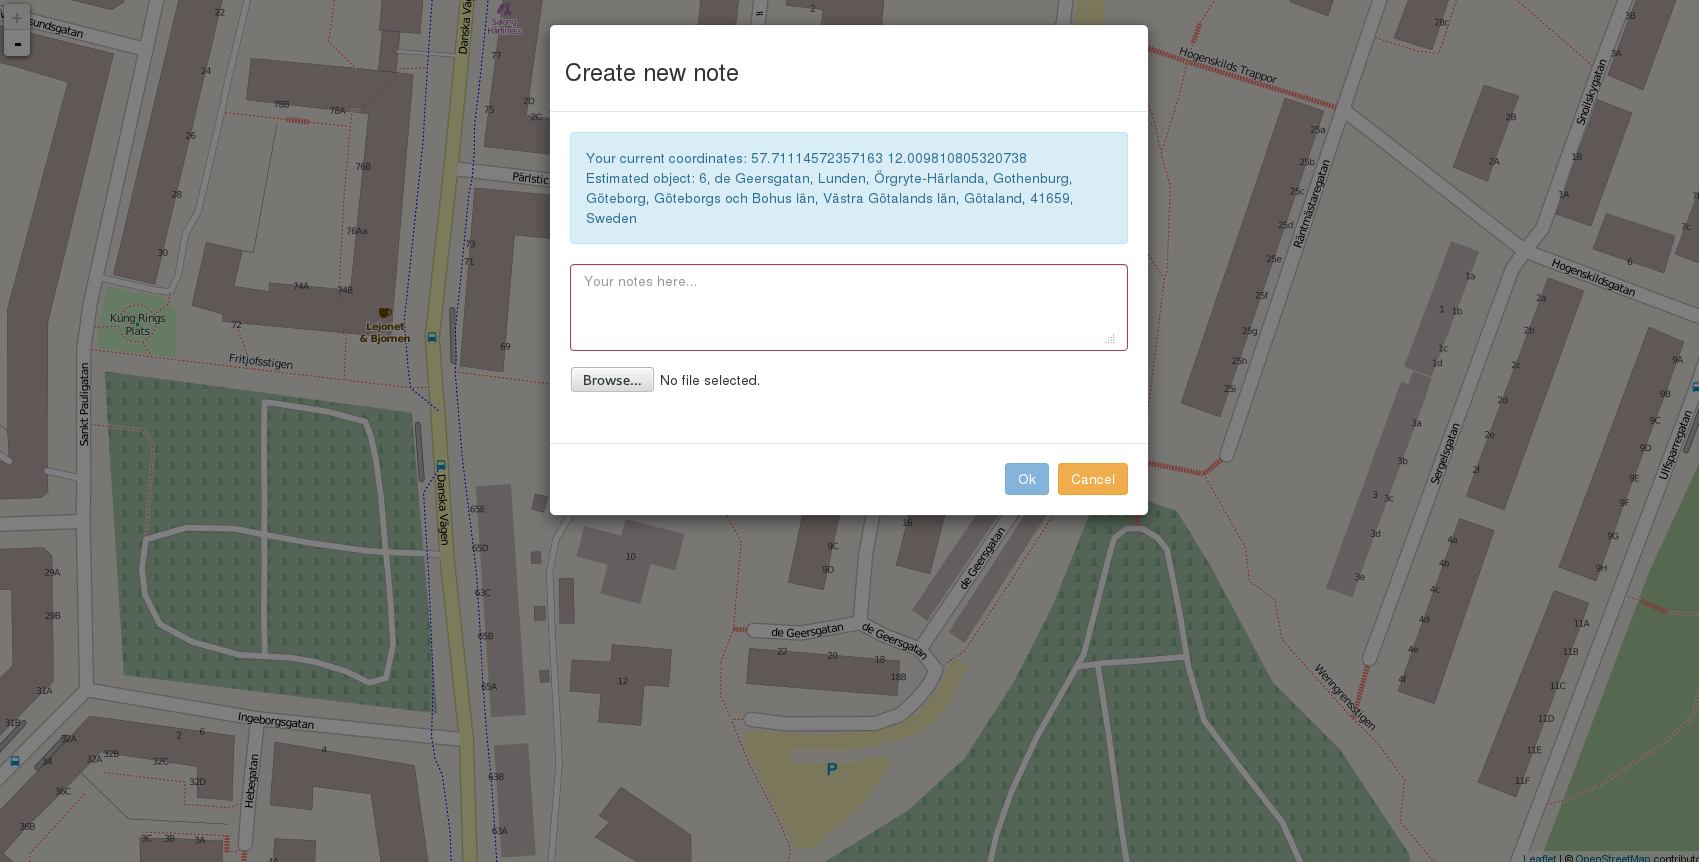
\includegraphics[width=\textwidth]{res/online}
      \end{center}
      \caption{Online version}
    \end{figure}

    \begin{figure}[h]
      \begin{center}
        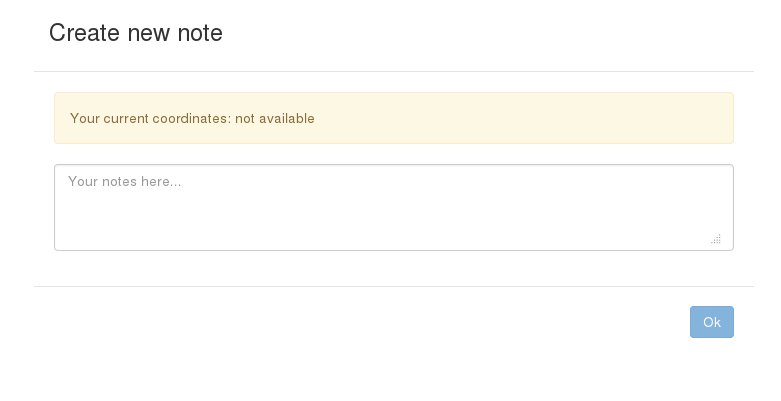
\includegraphics[width=\textwidth]{res/offline}
      \end{center}
      \caption{Offline version}
    \end{figure}

One of the neat features of AngularJs is good support for form validation and in overall
handling different form states (clean - dirty, valid - invalid). This allows to
easily give user feedback, whether he can submit the form or not and what is the problem.

EmberJs is the youngest from the three frameworks. It uses similar technics
as AngularJs, but with more ordinary javascript point of view, thus requiring
less mind-changing. Compare to other libraries, EmberJs has the largest file size,
because of including a lot of features into the standard build. It is great for
developing big sites, which has chances to use this features, but for the small
single-page application, devoted for the mobile use, it is not so great. Than is
why we decided to use AngularJs for this project, which has enough of useful
features, but is not overhelmed with them.

On the figures there are screenshots of offline version, which contains only form,
and on the other, this form embedded in modal dialog, which appears on click on map.

\subsection{Leaflet}

Leaflet is a JavaScript library for showing interactive maps. As a map
provider it utilizes OpenStreetMap and its derivatives, but can also
adopt data from Google Maps. Leaflet is designed with simplicity,
performance and usability in mind. It works efficiently across all
major desktop and mobile platforms out of the box, taking advantage of
HTML5 and CSS3 in modern browsers while maintaining compatibility with
the older ones.

Leaflet is relatively new project compared to OpenLayers. This means
Leaflet doesn't yet have a bloated codebase which makes it easier to
use; on the other hand though the documentation leaves much to be
desired, with examples and tutorials lagging behind. Leaflet's
community of developers is also still in its youth. For instance, the
Leaflet extension for AngularJS is quite immature, which results in
the necessity of either manually extending it for new cases, or
falling back to calling Leaflet directly.

Despite the previous statement, \textbf{leaflet-directive} is one of
the reasons we employed Leaflet if favor of the alternatives.
Leaflet-directive is a JS library that embeds Leaflet into AngularJS
concepts and idioms. It ensures that Leaflet map behaves and gets
managed as an idiomatic reactive entity.

Another principal advantage of Leaflet over OpenLayers in this
particular project is that the former is more suitable for the mobile
web. Leaflet is generally smaller and has a built-in support for
touch-screen events (touches are mapped to the clicks and you can zoom
map with two fingers without adding extra code). For OpenLayers we
would have to implement this features manually.

\subsection{Cache manifest}
For providing offline version HTML5 cache manifest file is used. It is still working
draft, but has support if most recent browsers (even in mobile, except Opera Mini).

Through special manifest file, application can specify which files are required for
offline version and should be cached. Useful feature is the \textbf{FALLBACK} section,
where you can specify the replacements for particular files, when there is no network
access.

Offline version of the application has two key files different from online.
It is \textit{app.js}, which is specification of Angular application, where root
controller is specified. For online version, root controller and template renders maps
and for offline version, it is just form, where user can write his notes.

Next is \textit{services.js}, which corresponds to the model. In offline version
it should save notes to the localstorage, in the online version - send requests
to the server.

\section{DropboxAPI}

To integrate with DropboxAPI we preferred server-side synchronization.
There were multiple reasons to support this decision:

\begin{itemize}
\item this approach conforms to RESTful design principles which state
  that a server can hide a N-tier architecture beneath.
\item it simplifies the client as the client doesn't have to deal with
  establishing and maintaining the connection to Dropbox.
\item security concerns - passing the Dropbox access token to the
  client creates a vulnerability which may result in a security breach.
\end{itemize}

Dropbox provides a well-designed API that can be accessed via OAuth
authorization. There are three types of API which the application can
use:

\begin{description}
\item[CoreAPI] - provides access to a regular file system. Allows to
  upload and download files.

\item[SyncAPI] - special API for native mobile apps, it can sync files
  and be notified of changes.

\item[DatastoreAPI] - gives access to a special storage, designed to
  hold raw data instead of files. Each datastore is a table of
  records. Each record is a set of key-value pairs where values can be
  strings, numbers etc.
\end{description}

An application that wants access any of the APIs listed should request
an app key and use this key in process of authorization. There are two
different types of permissions that the application can request: first
grants access only to the app folder and Datastore, and second gives
admission to all files of the user. For our project the first set of
permissions is sufficient.

Therefore our server-side application uses two Dropbox APIs: CoreAPI
and DatastoreAPI. CoreAPI is called to upload user media content (like
images). Synchronization of other data (like coordinates and text) is
performed via DatastoreAPI.

As a substitute for Dropbox to backup user data we considered
WebDAV\footnote{\url{http://webdav.org/}}. WebDAV is not a service but
an open protocol, an extension of HTTP that facilitates storing,
retrieving and collaborative editing of documents and files on World
Wide Web. We composed a list of advantages WebDAV-based solution has
over other similar services:

\begin{itemize}
\item Since the protocol is open, any open-source WebDAV-enabled
  server may be adopted (even the one that is self-hosted). Also the
  user of the API can be sure that there are no wiretapping bookmarks
  in the server code. This is especially significant in a post-Snowden
  era when data privacy once again becomes a crucial concern.
\item Also the openness of the protocol wins over proprietary
  solutions as it is easier to use the API and remove flaws when the
  specification and implementation of the storage server is publicly
  available.
\item The specification is stable, and the API won't suddenly change
  unlike it does in proprietary services.
\end{itemize}

In our experiment we tried WebDAV interaction with the already
configured ownCloud\footnote{\url{http://owncloud.org}} server.
ownCloud is a complex personal cloud solution which manages WebDAV,
CalDAV, CardDAV and other subservices. In order to communicate with
its WebDAV service, we added
python-webdav\footnote{\url{https://github.com/scaryclam/python-webdav}}
library to our server application, which is just a thin wrapper around
WebDAV HTTP requests. It provides a straightforward method to connect
and upload files to the WebDAV instance. In Python code it looks like
this:

\begin{lstlisting}[language=Python]
  import python_webdav.client
  ...
  c = python_webdav.client.Client('http://example.com/', '/myDir')
  c.set_connection(username='user', password='pass')
  response = c.upload_file('mydata.json')
\end{lstlisting}

Overall we found WebDAV to be more suitable for the task we were
facing. The only disadvantage when compared to Dropbox is the lack of
effective key-value storage (substitute for Datastore API). Because of
this fact we were forced to manipulate a JSON file and manually upload
it to the ownCloud server. The other point of difference is the
necessity of hosting the server yourself (which can be either
advantage or disadvantage, depending on the situation).

\section{Reverse geocoding}

Geocoding is the process of finding associated geographic coordinates
from other geographic data. In our project we used the technique of
reverse geocoding, when the geographic entity is resolved given its
coordinates as latitude and longitude. This information can be helpful
when the user creates a new note on the map - by seeing the exact
address of the created note he can ascertain that there are no mistake
with note location.

Since we already benefited from OpenStreetMap as the map provider, it was
consistent to use OSM as a geocoding source. Eventually we ended up
with Nominatim\footnote{\url{http://nominatim.openstreetmap.org}}, a simple
service running on top of OSM databases. Nominatim provides an API
accessed by HTTP GET request that returns data in the specified format
(JSON in our case).

One useful feature of Nominatim is the granularity of its results.
This means that the coarser the coordinates are in the request, the
more general the response will be. This synergizes rather well with
Leaflet, which when clicked upon gives back coordinates of different
accuracy based on the zoom factor. Therefore, if user clicks on the
map from a top view, Nominatim returns the name of the country and
probably city. But as the map is zoomed in more, geocoding source can
response with more precise information.

\section{Source code}
    You can find the latest version of the code on Github.
    \url{https://github.com/AAzza/geonaut}.

    \begin{description}
        \item[server/] here lives the restful server.
        \item[test\_server.py] here lives tests for server.
        \item[templates/manifest.appcache.jinja] Template for HTML5 cache manifest file.
        \item[static/index.html] entry point for the client-side.
        \item[static/js/app.js] entry point for the Angular applicaion.
        \item[static/js/app\_offline.js] entry point for the offline Angular applicaion.
        \item[static/js/controllers.js] file with all controllers, which contains all application logic.
        \item[static/js/services.js] storage and model for online version (perform request to server).
        \item[static/js/services\_offline.js] storage and model (store data to localstorage).
        \item[static/js/partial/] directory with html templates
    \end{description}
\end{document}
